
\chapter{Model of Solution System\label{chpt:models}}

Computing models of solvents are broadly divided into two types: those
treating the solvent as a continuous medium (implicit models) and
those describing the individual solvent molecules (explicit models).
In the continuum model, the solvent is characterized by the dielectric
constant $\varepsilon$ and contains an artificially shaped cavity.
The explicit models can have more specific microscopic scales. Within
the scope of classical mechanics, the most detailed (and thus the
most expensive) methods involve flexible and polarizable explicit
models, while in computational chemistry, less detailed models often
have wider usage (for example, the proteins are treated in the unity
of residues). As the theory of liquids was initially established for
spherical atom-like solvent particles, the model adopted by such a
theory is a rigid entity carrying distributed point charges, characterized
by their position and orientation, i.e. there is no internal movement
considered. This approximation has been proven reasonable \citep{Gray-Gubbins}.
There also exist models in which the scale lies somewhere between
the implicit and explicit models; for example, so-called coarse-grained
models \citep{hadley_coarse-grained_2012}, which gather groups of
atoms into a single interaction site.

In this section, we will give a brief introduction of the implicit
model in order to facilitate later discussion on solvation free energy
corrections. We will then focus on the rigid solvent models and discuss
the limits of such approximations. The flexible and polarizable models
will also be briefly mentioned. 

\section{Continuum solvation models}

Continuum models \citep{Jensen,Cramer_1999,Tomasi_1994_implicit_model},
which are popular in \acs{QM} calculations, consider the solvent
as a polarizable medium with dielectric constant $\varepsilon$\marginpar. The dielectric constant $\varepsilon$ is the key parameter characterizing
the solvent. It is normally a constant value, but that can depend
on the position in space (see $\mathsection$\ref{subsec:Poisson=002013Boltzmann-methods}), with the solute $M$ placed in the cavity within this medium (figure
\ref{fig:Reaction-field-model}). 

\begin{figure}[h]
\begin{centering}
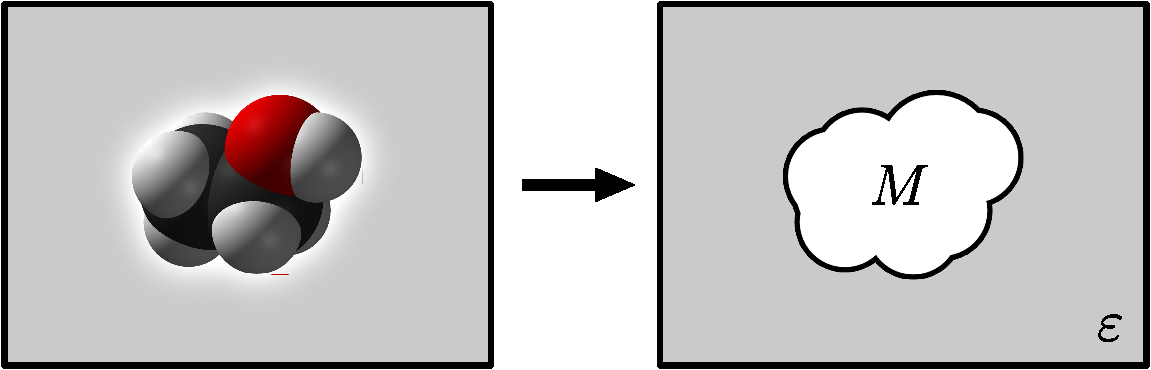
\includegraphics[width=0.72\columnwidth]{_figure/reaction-field-model_2}
\par\end{centering}
\caption{Continuum solvent model\label{fig:Reaction-field-model}}
\end{figure}

According to this model the solvation Gibbs free energy is
\begin{equation}
\Delta G_{\mathrm{solvation}}=\Delta G_{\mathrm{cavity}}+\Delta G_{\mathrm{dispersion}}+\Delta G_{\mathrm{elec}}\label{eq:Continuum-mod}
\end{equation}
where $\Delta G_{\mathrm{cavity}}>0$ is the energy needed to create
a hole in the medium, and $\Delta G_{\mathrm{dispersion}}$ is the
dispersion interaction, which is roughly the van der Waals energy
$\Delta G_{\mathrm{vdW}}<0$ between the solvent and solute. In principle,
there may also be a repulsive component, and the dispersion term is
sometimes denoted dispersion/repulsion. $\Delta G_{\mathrm{elec}}<0$
is the contribution of electrostatic interactions, introduced by electric
charge distribution of $M$ which polarizes the medium, and the action
back of the medium on the molecule (reaction field). 

The initial two terms in eq. (\ref{eq:Continuum-mod}) are linked
to the configuration of the first solvation shell (cavity). The definition
of cavity varies from the simplest sphere or ellipsoid to the ensemble
of atomic surfaces defined by the van der Waals radii in the solute.
It is somewhat reasonable to consider the cavity area as proportional
to the number of solvent molecules in the first solvation shell. This
number can be calculated as the area passing through the middle region
of first shell solvent. This area, named the solvent-accessible surface
area (SASA) \citep{SAS_1,SAS_2}, can be calculated by adding the
radius of the probe solvent ball to the solvent excluded surface area
(figure \ref{fig:sasa}).

\begin{figure}[h]
\begin{centering}
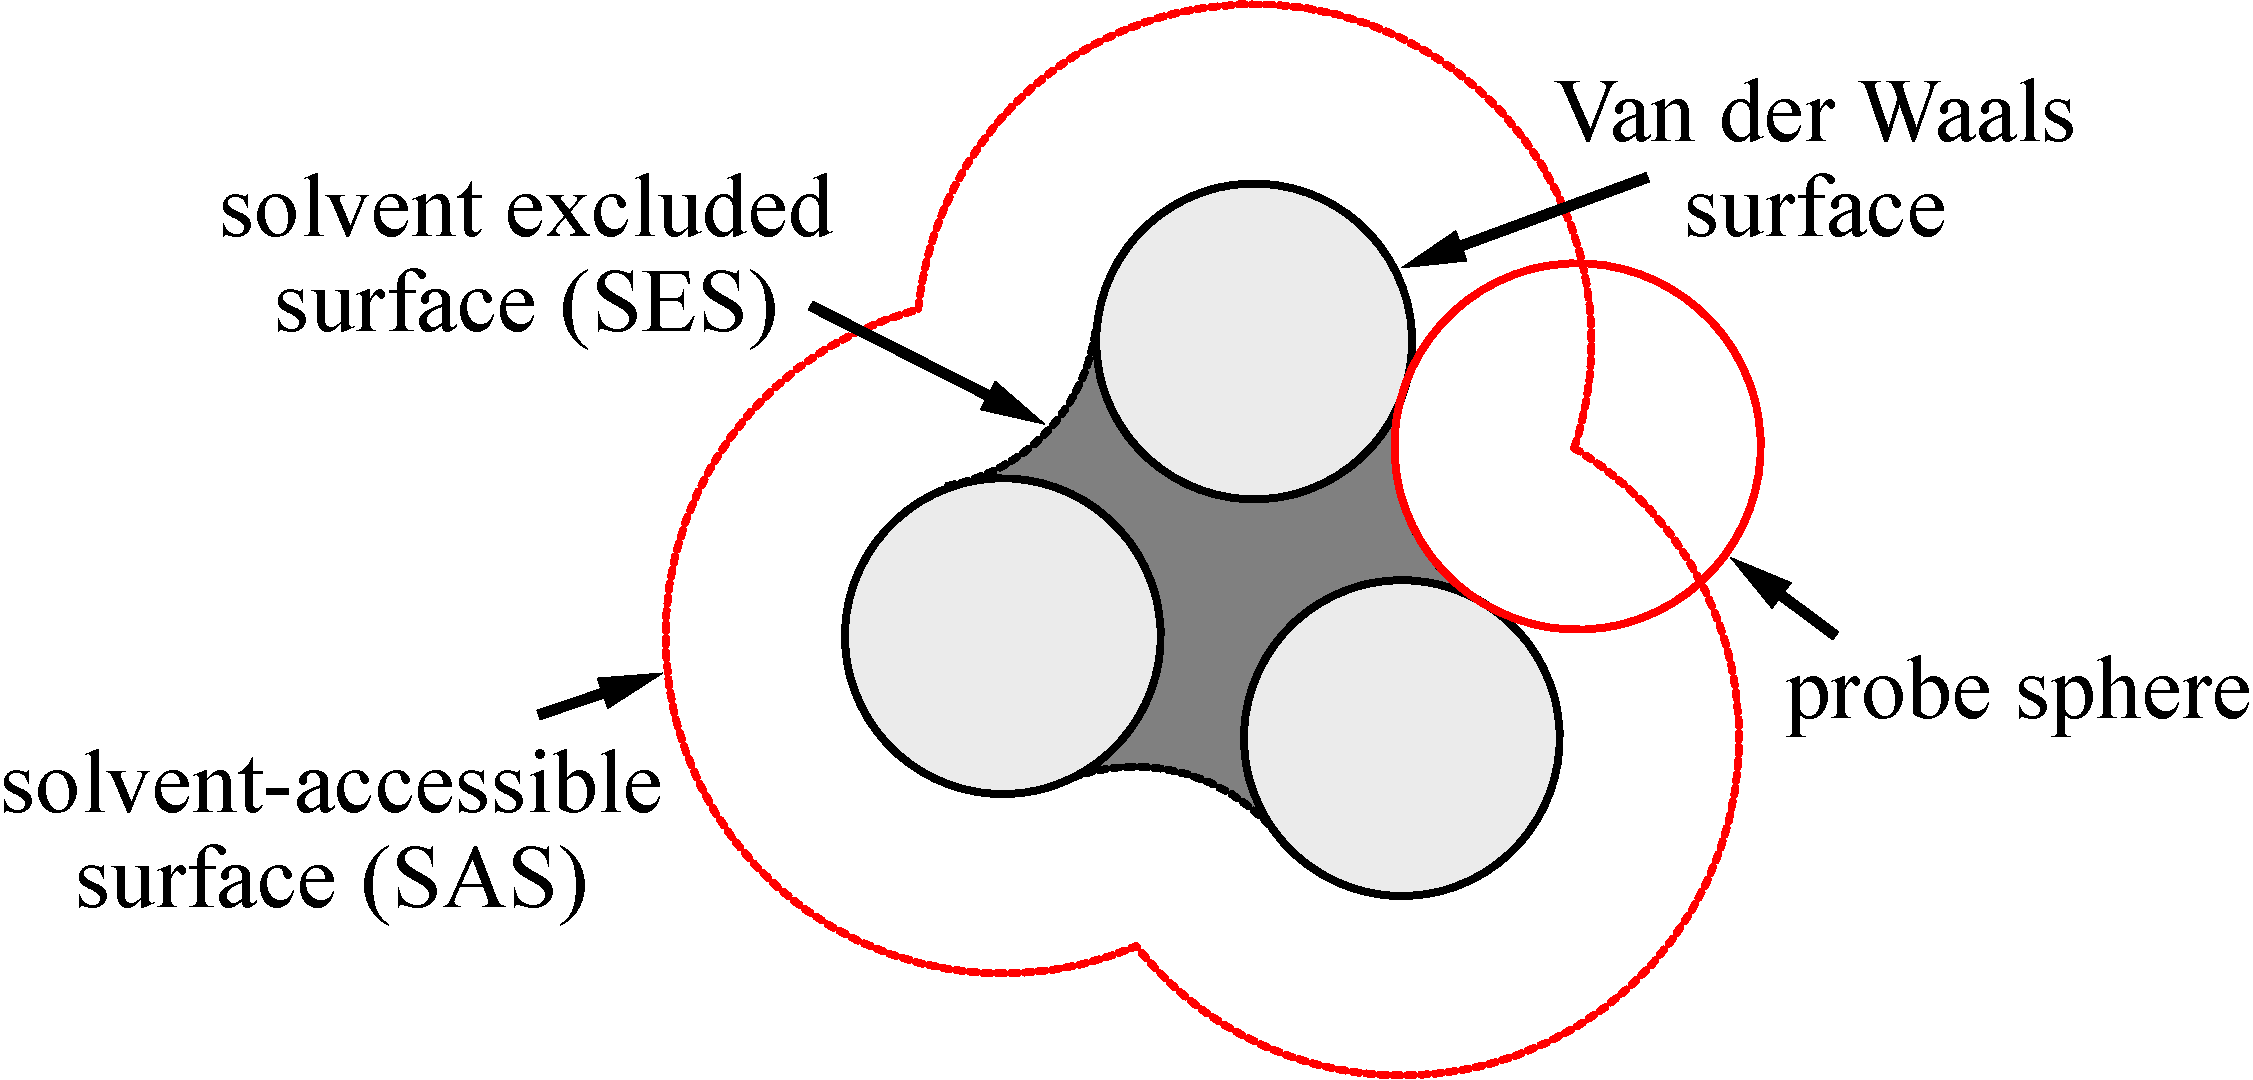
\includegraphics[width=0.55\columnwidth]{_figure/SASA}
\par\end{centering}
\caption[Definition of cavity surfaces]{Definition of cavity surfaces\label{fig:sasa}. The solvent accessible
surface (SAS) traced out by the center of the probe representing a
solvent molecule. The solvent excluded surface (SES) is the topological
boundary of the union of all possible probes that do not overlap with
the molecule.}
\end{figure}

The energy required to create such a cavity and the stabilization
due to van der Waals interactions between the solute and solvent,
assumed to be proportional to the surface area of the cavity, is expressed
as
\begin{equation}
\Delta G_{\mathrm{cavity}}+\Delta G_{\mathrm{dispersion}}=\gamma S_{\mathrm{SASA}}+\beta
\end{equation}
or parameterized by having a constant $\xi$ specific for each atom
type, with the $\xi$ parameters being determined by fitting to experimental
solvation data:
\begin{equation}
\Delta G_{\mathrm{cavity}}+\Delta G_{\mathrm{dispersion}}=\sum_{i}^{\mathrm{atoms}}\xi_{i}S_{i}
\end{equation}

The models and methods employed to calculate the electrostatic contribution
$\Delta G_{\mathrm{elec}}$ have varied greatly according to their
usage. The sections below list the most common examples. On another
topic, the integration of continuum models into \acs{QM} calculations
is also a very important field; these developments will not be detailed
here as they do not connect yet to our work. Such kinds of methods
are called the self-consistent reaction field (SCRF) models, which
integrate the calculation of the solute-solvent interaction in addition
to that of the solute wave function by an iterative procedure. Some
examples are presented in the list of Gaussian keyword SCRF \citep{scrf},
and the field is well reviewed by, for example, Tomasi \citep{Tomasi_1994_implicit_model,tomasi_quantum_2005}
and Jensen \citep{Jensen}.

\subsection{Poisson-Boltzmann methods\label{subsec:Poisson=002013Boltzmann-methods}}

The Poisson-Boltzmann equation (PBE) \citep{holst_1994_poisson} makes
it possible to calculate the position-dependent electrostatic potential
$V_{\mathrm{elec}}(\mathbf{r})$ in the continuum model, such that
the electrostatic component of the free energy can be written as
\begin{equation}
\Delta G_{\mathrm{elec}}=\frac{1}{2}\int\mathrm{d}\mathbf{r}\rho_{q}(\mathbf{r})V_{\mathrm{elec}}(\mathbf{r})
\end{equation}
where $\rho_{q}$ is the charge distribution of the solute.

The Maxwell-Gauss equation in SI units convention gives
\begin{equation}
\nabla\cdot D(\mathbf{r})=\dfrac{\rho_{q}(\mathbf{r})}{\varepsilon_{0}}
\end{equation}
where $D(\mathbf{r})=\varepsilon_{0}E(\mathbf{r})+P(\mathbf{r})$
is the electric displacement field, $P(\mathbf{r})$ is the system
polarization, $E(\mathbf{r})$ the electric field, and $\varepsilon_{0}$
the vacuum permittivity. $D(\mathbf{r})$ can also be expressed in
terms of the position-dependent dielectric constant $\varepsilon(\mathbf{r})$,
$D(\mathbf{r})=\varepsilon(\mathbf{r})E(\mathbf{r})$, which thus
gives
\begin{equation}
\nabla\cdot\varepsilon(\mathbf{r})E(\mathbf{r})=\dfrac{\rho_{q}(\mathbf{r})}{\varepsilon_{0}}
\end{equation}
or in terms of electrostatic potential:
\begin{equation}
\nabla\cdot\left[\varepsilon(\mathbf{r})\nabla V_{\mathrm{elec}}(\mathbf{r})\right]=-\dfrac{\rho_{q}(\mathbf{r})}{\varepsilon_{0}}\label{eq:poisson}
\end{equation}

This second-order differential equation (\ref{eq:poisson}) is called
the Poisson equation. 

This equation cannot be solved analytically for complex geometries
(such as a protein). Therefore it is done numerically using appropriate
methods; for example, as mentioned in the article of Roux and Simonson
\citep{roux_implicit_1999} or Holst \citep{holst_1994_poisson}.
A density functional approach based on the minimization of the polarization
density can also be used to solve this equation \citep{Marchi_2001,Levy_2005}.

If the solvent is ionic, the Poisson equation can be modified by taking
into account a (thermal) Boltzmann distribution of ions in the solvent,
i.e.,
\begin{equation}
\rho_{\mathrm{tot}}(\mathbf{r})=\rho_{q}(\mathbf{r})-2qn_{\mathrm{ion}}\sinh(\frac{q}{k_{\mathrm{B}}T}V_{\mathrm{elec}}(\mathbf{r}))
\end{equation}
for a salt composed of ions of charge $+\mathfrak{q}$ and $-\mathfrak{q}$
and of density $n_{\mathrm{ion}}$. Replacing in eq. (\ref{eq:poisson})
leads to the Poisson-Boltzmann Equation:
\begin{equation}
\nabla\cdot(\varepsilon(\mathbf{r})\nabla V_{\mathrm{elec}}(\mathbf{r}))-\dfrac{2qn_{\mathrm{ion}}}{\varepsilon_{0}}\sinh\left(\dfrac{qV_{\mathrm{elec}}(\mathbf{r})}{k_{\mathrm{B}}T}\right)=-\dfrac{\rho(\mathbf{r})}{\varepsilon_{0}}
\end{equation}


\subsection{Born / Onsager / Generalized Born models\label{subsec:Born-/-Onsager}}

For simple geometries, the Poisson equation (\ref{eq:poisson}) can
be solved analytically. The simplest model is a spherical cavity.
For a net charge $q$ in a cavity of radius $a$, the electrostatic
free energy of a medium with a dielectric constant of $\varepsilon$
is given by the Born formula:
\begin{equation}
\Delta G_{\mathrm{elec}}(q)=-\dfrac{1}{8\pi\varepsilon_{0}}\left(1-\frac{1}{\varepsilon}\right)\frac{q^{2}}{2a}\label{eq:born_model}
\end{equation}

Other similar models include the Onsager model, in which a point dipole
(characterized by the dipole moment $\mu$) is put in a spherical
cavity. The Kirkwood model refers to a general multipole expansion
in a spherical cavity, while the Kirkwood-Westheimer model arises
for an ellipsoidal cavity. Those simplified models are not fully able
to predict the solvent behavior in many realistic cases \citep{Jensen}. 

The generalized Born (GB) model is an empirical model based on the
superposition of several net charges in spherical cavities as the
Born model describes, with a similar formula:
\begin{equation}
\Delta G_{\mathrm{elec}}=-\dfrac{1}{8\pi\varepsilon_{0}}\left(1-\frac{1}{\varepsilon}\right)\sum_{i}\sum_{j}\frac{q_{i}q_{j}}{f_{ij}}
\end{equation}
where the function $f_{ij}$ depends on the internuclear distance
$r_{ij}$ between the centers of atoms $i$ and $j$ and on the Born
radii for each pair of atoms $a_{i}$ and $a_{j}$:
\begin{equation}
f_{ij}=\sqrt{r_{ij}^{2}-a_{i}a_{j}\exp\left(\frac{r_{ij}^{2}}{4a_{i}a_{j}}\right)}
\end{equation}

The key (empirical) point is to be able to attribute an effective
Born radius $a_{i}$ to each atom inside the complex, non-spherical
cavity formed by the solute. Once this is accomplished, the GB model
provides a very fast method, with an overall accuracy comparable to
that of Poisson-Boltzmann calculations. That makes it widely used
in computational structural biology to perform structure optimization
and molecular dynamics simulations.

\section{Model potential of explicit molecules\label{sec:rigid-model-potential}}

The model potential frequently used in the theory of liquids is a
classical, rigid, pairwise additive model \citep{Hensen-McDonald,Gray-Gubbins}.
It is based on three assumptions. 
\begin{enumerate}
\item Firstly, the quantum effects should be ignored. It is assumed that
the rotational and transitional motion of solvent particles are continuous
and classical, which means the separation of both transitional and
rotational states are largely inferior of $k_{\mathrm{B}}T$. For
light molecules, that is not always convincing. Some molecules containing
hydrogen (e. g. $\mathrm{H_{2}O}$, $\mathrm{NH_{3}}$, and particularly
$\mathrm{H_{2}}$) exhibit obvious quantum effects at low temperatures
in the liquid state. Gaseous $\mathrm{H_{2}O}$ and $\mathrm{NH_{3}}$
also need quantum effect corrections. However, for the liquid of most
interest to us, $\mathrm{H_{2}O}$ at room temperature, the contribution
of this effect is small enough to be neglected. And obviously, there
should not be any chemical interaction of the solvent with the solute.
\item Secondly,\marginpar{compared to atomic models that only depend on $\mathbf{r}^{N}$, the
angular correlations can give influence on both structural and thermodynamic
proprieties. That is why our theory is extended to linear case, $\mathbf{\Omega}\equiv(\Theta,\Phi)$,
then molecular case, $\mathbf{\Omega}\equiv(\Theta,\Phi,\Psi)$.} The intramolecular movement (vibration and internal rotation) should
be either independent of transitional and rotational movement or absent.
This rigid molecule approximation assumes that the intermolecular
potential $\mathcal{U}(\mathbf{r}^{N},\mathbf{\Omega}^{N})$ for $N$
particles only depends on the positions of the $N$ molecular centers
$\mathbf{r}^{N}\equiv(\mathbf{r}_{1},\mathbf{r}_{2},\ldots,\mathbf{r}_{N})$
and on their orientations $\mathbf{\Omega}^{N}\equiv(\mathbf{\Omega}_{1},\mathbf{\Omega}_{2},\cdots,\mathbf{\Omega}_{N})$,
where $\mathbf{\Omega}\equiv(\Theta,\Phi,\Psi)$ represents the Euler
angles (figure \ref{fig:Euler-angles}). The natural choice for the
molecular center is the center of mass. This is, however, arbitrary
if only equilibrium properties are considered.

\begin{figure}[h]
\begin{centering}
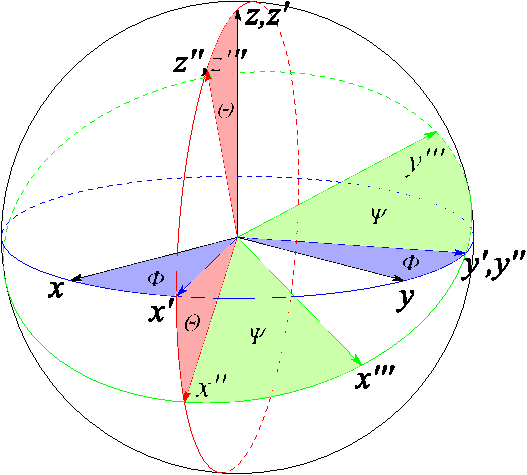
\includegraphics[scale=0.75]{_figure/euler_sphere}
\par\end{centering}
\caption[Euler angles]{Euler angles. The basis vectors of the new orientation are obtained
by 3 sequential operations: (1) A rotation $\phi$ $(0<\phi<2\pi)$
about the $z$-axis, bringing the frame of axes from the initial position
$\mathbf{S}$ into the position $\mathbf{S}'$ (2) A rotation $\theta$
$(0<\theta<\pi)$ about the $y$-axis of the frame $\mathbf{S}'$,
which is transformed into $\mathbf{S}''$ (3) A rotation $\psi$ $(0<\psi<2\pi)$
about the $z$-axis of the frame $\mathbf{S}''$.\label{fig:Euler-angles}}
\end{figure}

The rigid approximation is quite realistic for molecules in which
the separation of vibrational states largely exceeds $k_{\mathrm{B}}T$,
implying that the molecule stays in its ground vibrational state.
This is the case for many small solvent molecules such as $\mathrm{N_{2}}$,
$\mathrm{CO_{2}}$, $\mathrm{C_{6}H_{6}}$, and indeed for the bending
and stretching modes of water. 
\item Finally, the intermolecular forces have to be assumed as pairwise
additive:
\begin{equation}
\mathcal{U}(\mathbf{r}^{N},\mathbf{\Omega}^{N})=\frac{1}{2}\sum_{i\neq j}u(\mathbf{r}_{ij},\mathbf{\Omega_{i}},\mathbf{\Omega_{j}})=\sum_{i<j}u(\mathbf{r}_{ij},\mathbf{\Omega_{i}},\mathbf{\Omega_{j}})\label{eq:pair-potential}
\end{equation}
This means that the model potential only depends on the intermolecular
separation $\mathbf{r}$ and on the molecular orientations $\mathbf{\Omega}_{1}$
and $\mathbf{\Omega}_{2}$. This approximation is quasi-exact for
low density gases, where the contribution of the three and more body
terms decreases rapidly. But for dense fluids, in most of the cases
the multi-body potential cannot be ignored. The complete model potential
with higher-order corrections can be written in the form of
\begin{equation}
\mathcal{U}(\mathbf{r}^{N},\mathbf{\Omega}^{N})=\sum_{i<j}u(ij)+\sum_{i<j<k}u(ijk)+\sum_{i<j<k<l}u(ijkl)+...
\end{equation}
where $u(ij)=u(\mathbf{r}_{ij},\mathbf{\Omega_{i}},\mathbf{\Omega_{j}})$
and $u(ijk)=u(\mathbf{r}_{ij},\mathbf{r}_{jk},\mathbf{r}_{ki},\mathbf{\Omega_{i}},\mathbf{\Omega_{j}},\mathbf{\Omega_{k}})$,
etc. The omission of the three-body and higher-order terms can cause
errors, for example, in surface tension and surface energy calculation
\citep{Miyazaki_1975}. However the higher order terms are often accounted
for by an effective pair potential (measured by experiments or calculated
by simulations), which reduces considerably the computational cost
for simulations, or the degree of theory needed. Such models are presented
below, going from simple to molecular liquids. For the molecular solvent
considered in this thesis, water, most publications have stayed at
this two-body level of description. 
\end{enumerate}

\subsection{Interaction of spherical particle}

The simplest model of a fluid is the hard sphere model. With $d$
the hard-sphere diameter, the pair potential is defined as:
\begin{equation}
u(r)=\begin{cases}
\infty & r<d\\
0 & r>d
\end{cases}
\end{equation}
This model is indeed a fundamental reference model in statistical
mechanics, and it can represent some physical systems, such as neutral
colloidal suspensions \citep{Cohen1998251}. However, the absence
of attractive force, which precludes the existence of a liquid-gas
transition, makes it too simple for realistic fluids. More realistic
neutral particle models, like the Lenard-Jones (LJ) model, exhibit
a potential energy curve that has the same shape as the real interaction
of rare gas, as shown in figure \ref{fig:LJ-pair-potential}.

\begin{figure}[h]
\begin{centering}
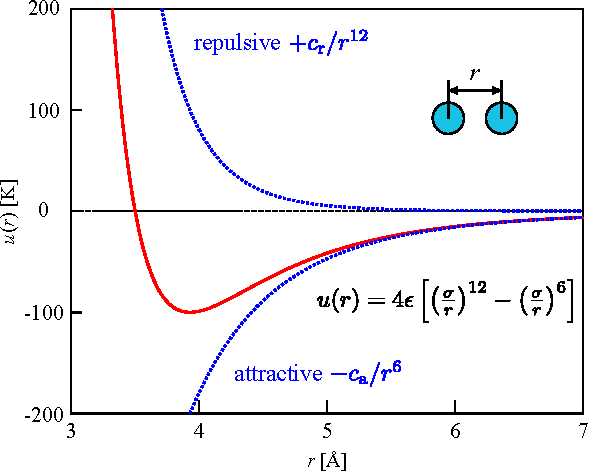
\includegraphics[scale=0.82]{_figure/lj-centre}
\par\end{centering}
\caption[LJ pair potential]{LJ pair potential. The plot gives the potential energy $u(r)$ versus
internuclear distance $r$ of two particles. At large distances, both
attractive and repulsive interactions are small. As the distance between
the atoms decreases, the attractive electron-proton interactions dominate,
and the energy of the system decreases. At the observed bond distance,
the repulsive electron-electron and proton-proton interactions just
balance the attractive interactions, preventing a further decrease
in the internuclear distance. At very short internuclear distances,
the repulsive interactions dominate, making the system less stable
than the isolated atoms.\label{fig:LJ-pair-potential}}
\end{figure}

The Lennard-Jones (LJ) interaction gives
\begin{equation}
u_{LJ}(r)=4\varepsilon\left[\left(\frac{\sigma}{r}\right)^{12}-\left(\frac{\sigma}{r}\right)^{6}\right]
\end{equation}
where $r$ is the distance from centre to centre, $\sigma$ is the
collision diameter or the particles separation where $u(r)=0$, and
$\epsilon$ is the well depth of the potential (of unity of energy).
The well minimum occurs at $r_{\min}=2^{1/6}\sigma$ and $u(r_{\min})=-\epsilon$.
The parameters $\sigma$ and $\epsilon$ can be extracted from experiments.

Theoretically, all terms in the multipole series represent attractive
contributions to the potential. The leading term, varying as $r^{-6}$,
describes the quantum dipole-dipole interaction. Higher-order terms
represent dipole-quadrupole ($r^{-8}$), quadrupole-quadrupole ($r^{-10}$)
interactions, and so on, but these are negligible compared to $r^{-6}$.
The short-range interaction is difficult to define properly, and for
the sake of simplicity and numerical efficiency, it is defined as
$r^{-12}$ in the LJ model. 

If the spherical particles are charged (as in molten salts), the electrostatic
interaction between them is described by the Coulomb point charge
interaction:
\begin{equation}
u_{\mathrm{Coul}}(r)=\frac{q_{1}q_{2}}{4\pi\varepsilon_{0}r}
\end{equation}

For such charged simple fluids, the overall pair $u(r)$ is a sum
of LJ and Coulomb interactions. Such decomposition can be extended
to molecular fluids in terms of site-site interactions, which are
discussed in the following section.

\subsection{Site-site interactions}

Indeed, a spherical description of interactions is not sufficient
to fully describe molecular fluids. The site-site model is a further
extension of atomic models in which the solvent molecule is represented
by a set of discrete interaction sites. The total potential energy
is a sum of spherical interaction potentials:
\begin{equation}
u(1,2)=\sum_{\alpha}\sum_{\beta}u_{\alpha\beta}(\left|\mathbf{r}_{2\beta}-\mathbf{r}_{1\alpha}\right|)
\end{equation}
where $\mathbf{r}_{is}$ is the coordinates of site $s$ in molecule
$i$, $u_{\alpha\beta}(r)$ the interatomic potential energy of pairs
of sites $\alpha$ and $\beta$, as discussed above. More specifically,
it is generally decomposed into a Lennard-Jones and a Coulombic contribution:
\begin{equation}
u(1,2)=\sum_{\alpha}\sum_{\beta}\left\{ 4\epsilon_{\alpha\beta}\left[\left(\frac{\sigma_{\alpha\beta}}{r_{12}^{\alpha\beta}}\right)^{12}-\left(\frac{\sigma_{\alpha\beta}}{r_{12}^{\alpha\beta}}\right)^{6}\right]\:+\frac{1}{4\pi\varepsilon_{0}}\frac{q_{\alpha}q_{\beta}}{r_{12}^{\alpha\beta}}\right\} 
\end{equation}
where $r_{12}^{\alpha\beta}=\left|\mathbf{r}_{2\beta}-\mathbf{r}_{1\alpha}\right|$,
$\epsilon_{\alpha\beta}$ and $\sigma_{\alpha\beta}$ are the site-site
LJ parameters and $q_{\alpha}$ the partial charge on each site. This
model is the most commonly adopted, and it will be so in this thesis
for the calculation of external free energy functional.

\subsection{Multipole and spherical harmonic expansion}

To obtain fewer terms in the calculation, the model potential can
be presented in convergent series via multipole or spherical harmonic
expansion.

For polar liquids, the dipole-dipole interaction should be mainly
taken into account. Thus the model considers dipole-dipole interactions
in addition to a spherically symmetric Lennard-Jones-like potential:
\begin{equation}
u(1,2)=u_{0}(r)-\boldsymbol{\mu}_{1}\cdot\mathbf{T}(\mathbf{r})\cdot\boldsymbol{\mu}_{2}
\end{equation}
where $\mathbf{r}$ is the vector separation of the molecular centers,
$u_{0}(r)$ is the spherically symmetric term discussed above, $\boldsymbol{\mu}_{i}$
is the dipole moment vector of particle $i$ and $\mathbf{T}(\mathbf{r})$
is the dipole-dipole interaction tensor:
\begin{equation}
T(\mathbf{r})=\nabla^{2}\left(\dfrac{1}{r}\right)=3\mathbf{r}\mathbf{r}/r^{5}-\mathbf{I}/r^{3}
\end{equation}
and $\mathbf{I}$ is the unit tensor. Note that this model can be
made more realistic by including higher-order electrostatic interactions,
such as dipole-quadrupole, quadrupole-quadrupole, etc. Such a systematic
multipolar approach has previously been proposed for water \citep{Chowdhuri_2006}.

Alternatively, the intermolecular potential can be expanded onto rotational
invariants in the form:
\begin{equation}
u(\mathbf{r}_{12},\mathbf{\Omega}_{1},\mathbf{\Omega}_{2})=\sum_{mnl\mu\nu}u_{\mu\nu}^{mnl}(r_{12})\Phi_{\mu\nu}^{mnl}(\hat{\mathbf{r}}_{12},\mathbf{\Omega}_{1},\mathbf{\Omega}_{2})
\end{equation}
where the angular basis functions $\Phi_{\mu\nu}^{mnl}(\hat{\mathbf{r}}_{12},\mathbf{\Omega}_{1},\mathbf{\Omega}_{2})$
can be expressed in terms of generalized spherical harmonics (\acs{GSH}s)
\citep{Gray-Gubbins}. A detailed description of rotational invariant
transform is in appendix \ref{chpt:rotational-invariant-expansion}.

\subsection{SPC/E water model}

As water cannot be perfectly described by a pair potential (due to
multi-body effects, quantum effects, hydrogen bond, etc.), various
models have been developed to fit a maximum number of properties.
Those models contain several sites, which can be placed possibly elsewhere
than at the center of atoms (figure \ref{fig:Water-models}). The
more sites the model has, the more precise it can be. There is a great
work done by Martin Chaplin \citep{water-model} to summarize the
most widely used water models.

\begin{figure}[h]
\begin{centering}
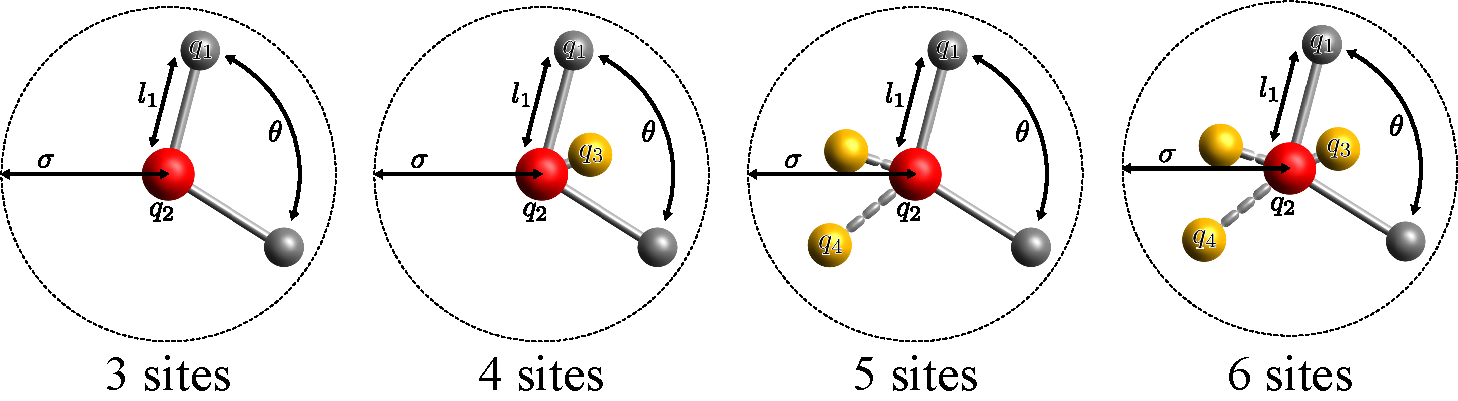
\includegraphics[width=0.85\columnwidth]{_figure/water}
\par\end{centering}
\caption{Water models\label{fig:Water-models}}
\end{figure}

In this thesis, we use the extended simple point charge model (SPC/E)
of water \citep{SPC/E} as our solvent model throughout.
It is a 3-site model, the electrostatic interaction being modeled
using Coulomb's Law and the dispersion and repulsion forces using
the Lennard-Jones potential, as described above. 

With respect to the original SPC model, the SPC/E model takes into
account the polarization in an implicit and phenomenological way,
re-normalizing the dipole of the effective pair model, and thus increasing
the partial charge slightly compared to SPC (table \ref{tab:SPC/E};
the center of water molecule has been placed at atom O, for convenance).
The SPC/E model gives a better radial distribution function and diffusion
constant than the SPC model. It is the most commonly used model for
applications.\marginpar{It should be noted that any rigid solvent model is compatible with
the theory that this thesis is base on, e.g. acetonitrile used in \citep{Zhao_2011}.}

\begin{table}[h]
\begin{centering}
\begin{tabular*}{1\columnwidth}{@{\extracolsep{\fill}}lllllll}
\toprule 
\tableheadline{Model} & $\sigma$ $[\lyxmathsym{\AA}]$ & $\varepsilon$ $[\mathrm{kJ\cdot mol^{-1}}]$ & $l_{1}$ $[\text{\AA}]$ & $\mathfrak{q}_{1}$ $[q_{e}]$ & $\mathfrak{q}_{2}$ $[q_{e}]$ & $\theta$ $[\text{\textdegree}]$\tabularnewline
\midrule
SPC \citep{spc} & 3.166 & 0.650 & 1.0000 & +0.410 & -0.8200 & 109.47\tabularnewline
SPC/E \citep{SPC/E} & 3.166 & 0.650 & 1.0000 & +0.4238 & -0.8476 & 109.47\tabularnewline
\midrule 
experiment \citep{water_exp} & - & - & 0.991 & - & - & 105.5\tabularnewline
\bottomrule
\end{tabular*}
\par\end{centering}
\caption{Structural parameters of SPC and SPC/E water\label{tab:SPC/E}}
\end{table}


\subsection{Flexible and polarizable models}

Up to this point, molecules were considered as rigid bodies. Flexible
models give extra degrees of freedom in vibration and internal rotation.
In that case, the interaction potential contains several extra terms,
yielding typically five kinds of forces: three for the direct interactions
in addition to the two indirect interactions (LJ and Coulomb).

\begin{figure}[h]
\begin{centering}
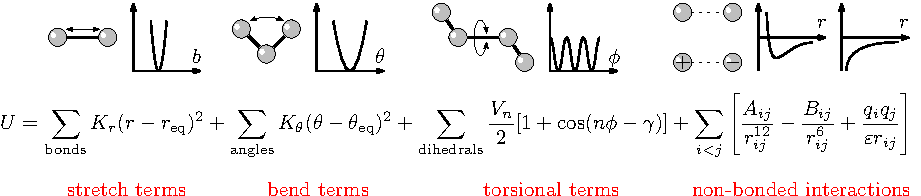
\includegraphics[width=1\columnwidth]{_figure/flexible}
\par\end{centering}
\caption{Interactions in a flexible model}
\end{figure}

The flexible yielding can deal with the non-rigidity of the solvent,
which is partially polarized owing to the vibrational degrees of freedom
(the so-called atomic polarizability). On the other hand, electronic
polarizability (the deformation of the molecule electron cloud under
the action of the external electric field) can be taken into account
even in a rigid model. This polarizability can be described by introducing
a modifiable charge distribution, for example by adding an induced
dipole at the molecular center of the molecule, or even on each of
its atomic sites, and by solving the set of induced dipoles self-consistently.
Introducing variable atomic charges is possible too \citep{Berne_1994}.
Optimizing the induced charges/dipoles has a large computational overhead
compared to fixed charges.

Complex models require expensive computing cost, but still can have
large fluctuations due to use of imposed small system size. There
is a compromise between the choice of model and the choice of system
size. For this reason, the rigid models are still the most
popular nowadays. On the other hand, computing technologies have greatly developed
compared to the theories themselves, which makes it possible to use
more and more precise models in computation. 

\section{Model of solute}

The model of solute also has a substantial influence on the predicted
energy and structure of solvation. The solute can eventually be treated
by \acs{QM} calculations in terms of wave function and electron density.
This is the case for the implicit SCRF method, which for apolar solvents
(i.e. toluene) has been proven to work well. There is a clear mismatch,
however, between the very refined description of the solute and the
rather primitive continuous-medium treatment of the solvent. The compromise
to have a better model of solvent or solute is debatable, and should
vary according to the applications. On the other extreme, one never
uses a quantum solvent model with an implicit solute; this would not
be profitable even if the solute is of simple geometry (wall). In
the case of molecular solutes, it is consistent to require the solute
to have at least the same scale of description as the solvent. A hierarchy
of possible potential models for solutes is described in figure (\ref{fig:Hierarchy-of-models}).
\begin{figure}[h]
\centering{}%
\noindent\begin{minipage}[t]{1\columnwidth}%
\begin{center}
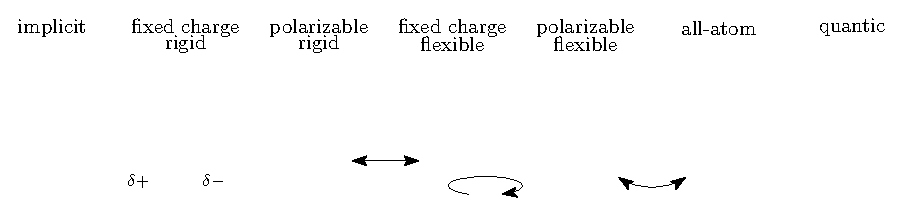
\includegraphics[width=1\columnwidth]{_figure/solute}
\par\end{center}%
\end{minipage}\caption{Hierarchy of solute models\label{fig:Hierarchy-of-models}}
\end{figure}

In this thesis, our first step will be to use a rigid molecular model
to describe the solute. This is coherent with IET, which cannot treat
the solvent and solute at different scales of description. Polarizable
and/or flexible models of solute, and the coupling of a \acs{QM}
solute to the molecular solvent, will be described in perspective.

In conclusion, the choice of model for the solute/solvent system is
a compromise between the required precision according to the application,
and the computing cost that the research can afford.
